\chapter{System architecture}
\label{cha:4}

Soweego is a pipeline that accomplishes several tasks in order to link entities between Wikidata and the target database. For the purpose of the following description, the target database will be MusicBrainz.\footnote{\url{https://musicbrainz.org}} MusicBrainz is a community-maintained open source encyclopedia of music information.\footnote{\url{https://musicbrainz.org/doc/About}} In particular, the relevant data for the pipeline are the artists, since they're humans.
\todo{Va esteso?}

\section{Importer}
\label{cha:41}
The importer is the pipeline's module in charge of downloading the latest target database dump and store it in a database. The import phase does not work on the data as is, but treats it to extract only the desired slice. Since soweego aims to work against different databases, there's a configurable middleware that handles the translation from the desired database to the project's format. The format consists in a set of basic attributes:
\begin{itemize}
    \item \textit{Catalog ID}, the identifier of the entity in the target database
    \item \textit{Label}, the full name
    \item \textit{Birth Date}
    \item \textit{Birth date precision}
    \item \textit{Death Date}
    \item \textit{Death date precision}
\end{itemize}
The schema is extendable for each source database, however the set of shared attributes enables having procedures in common among all the sources.

A common issue, in music databases above all, is people having   multiple names, known as \textbf{aliases}. The schema easily handles them by treating the aliases as standalone people. Clearly these standalone records will share all the original name's data, except the label.

BaseLink -> magari piccolo ER

Mapping di Musicbrainz


\section{Linker}
\label{cha:42}

Al momento sistema rule based per creare una baseline

Perfect name

birth and death dates

Damerau-Levenshtein

Levenshtein

Jaro-Winkler

Cross catalog link (including sitelinks)

Extension Token similarity for urls



\section{Ingestor}
\label{cha:43}

\section{Validator}
\label{cha:44}

\begin{figure}
  \begin{center}
   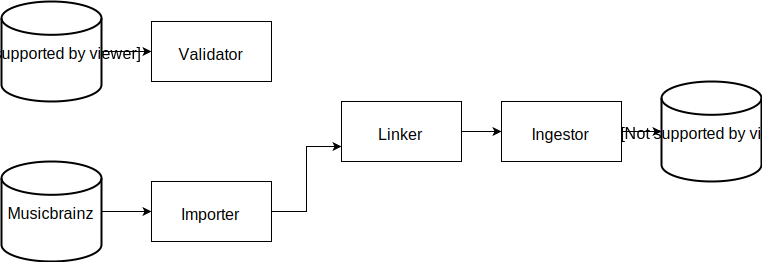
\includegraphics[width=\textwidth]{images/architecture.pdf}
   \captionof{figure}{Soweego architecture overview}
  \end{center}
\end{figure}

